\documentclass{article}
\usepackage{graphicx}
\begin{document}
  \title{Footnotes test}
  \author{Carl Capybara\footnote{Footnotes in author are displayed directly below author.}\footnote{They're quite often used for institutions and so on. We also don't want them to collide with the abstract.}}
  \maketitle
  \begin{abstract}
    A footnote test.
  \end{abstract}
  Lorem ipsum dolor sit amet, consectetur adipisicing elit, sed do eiusmod tempor incididunt ut labore et dolore magna aliqua. Ut enim ad minim veniam, quis nostrud\footnote{Footnotes inline in a paragraph are no problem.} exercitation ullamco\footnote{Another nearby will stack underneath the previous one.} laboris\footnote{And they should keep on stacking across the next paragraph instead of pushing it down.} nisi ut aliquip ex ea commodo consequat. Duis aute irure dolor in reprehenderit in voluptate velit esse cillum dolore eu fugiat nulla pariatur. Excepteur sint occaecat cupidatat non proident, sunt in culpa qui officia deserunt mollit anim id est laborum.

  Lorem ipsum dolor sit amet, consectetur adipisicing elit, sed do eiusmod tempor incididunt ut labore et dolore magna aliqua. Ut enim ad minim veniam, quis nostrud exercitation ullamco laboris nisi ut aliquip ex ea commodo consequat. Duis aute irure dolor in reprehenderit in voluptate velit esse cillum dolore eu fugiat nulla pariatur. Excepteur sint occaecat cupidatat non proident, sunt in culpa qui officia deserunt\footnote{Footnotes can have \emph{formatting}.} mollit\footnote{A stacked footnote should push figures down, not collide with them.} anim id est laborum.

  \begin{figure}[h]
    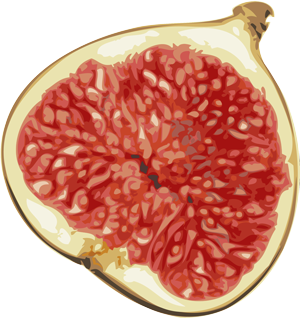
\includegraphics[width=8cm]{fig.png}
    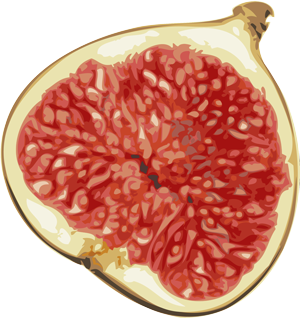
\includegraphics[width=8cm]{fig.png}
    \caption{Fig.}
    \label{fig:fig}
  \end{figure}
\end{document}
